\documentclass[conference]{IEEEtran}

\usepackage{amsmath}
\usepackage{amsfonts}
\usepackage{amssymb}
\usepackage[margin=1in]{geometry}
\usepackage{times}
\usepackage{setspace}
\usepackage{graphicx}
\usepackage{hyperref}
\usepackage[numbers]{natbib}
\usepackage{nomencl}
\usepackage{fancyhdr}

\begin{document}

\renewcommand{\abstractname}{ABSTRACT}
\title{Visually Programming a Robot}

\author{
\IEEEauthorblockN{Madhav Rao}
\IEEEauthorblockA{International Institute of \\Information Technology-Bangalore,\\
				  India 560100\\
				  mr@iiitb.ac.in}
\and
\IEEEauthorblockN{Rahul R}
\IEEEauthorblockA{International Institute of \\Information Technology-Bangalore,\\
				  India 560100\\
				  rahul.r@iiitb.org}}
\maketitle
\thispagestyle{plain}
\pagestyle{plain}
\renewcommand{\headrulewidth}{0pt}
\renewcommand{\footrulewidth}{0pt}

\begin{abstract}
This paper discusses on how to overcome the challenges of introducing a programming language to a beginner and to focus more on creative and fun part of programming. We propose a visual approach to programming where a programmer need not remember any of the constructs of a programming language, but only on the approach to solve a problem. We also extend the idea of using robotics in programming by using a real robot instead of a virtual robot simulator and thus giving a platform to learn fundamentals of object oriented programming as well as robotics.
\end{abstract}

\section{Introduction}
Let’s consider a simple problem to display “Hello World” on your console. Following are the programs in three popular programming languages C, Java and Python.

\begin{figure}[h]
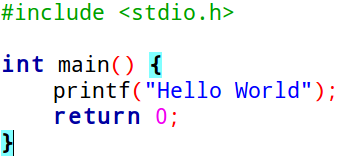
\includegraphics[scale=0.4]{Fig_01.png}
\caption{Hello World progrm in C}
\end{figure}

\begin{figure}[h]
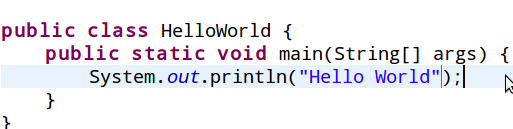
\includegraphics[scale=0.4]{Fig_02.png}
\caption{Hello World progrm in Java}
\end{figure}

\begin{figure}[h]
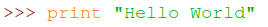
\includegraphics[scale=0.4]{Fig_03.png}
\caption{Hello World progrm in Python}
\end{figure}

Consider the C program. Isn't it a challenging task to explain the concepts of main, preprocessor directive, header file and return type to a programmer who writes this as his first program? The Java program too involves concepts of class, access modifier, static keyword and method call. The Python program is more intuitive than C or Java. Still a novice programmer has to remember that it’s not \texttt{print Hello World}  or \texttt{display "Hello World"} but it is \texttt{print "Hello World"}. 

In 1970s, Rich Pattis of Stanford University designed an introductory program environment where students control a virtual robot named Karel~\cite{karel}, to do simple tasks. Owing to the success of Karel, Stanford University adopted this robot simulator model in mid 90’s, to be a part of their curriculum to introduce principles of objected oriented programming using Java.

\begin{figure}[h]
\centering
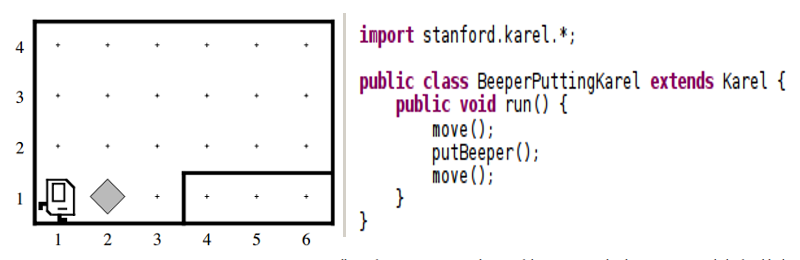
\includegraphics[scale=0.2]{Fig_04.png}
\caption{Karel and his world}
\end{figure}

This paper discusses on how to overcome the challenges of introducing a programming language to a beginner and to focus more on creative and fun part of programming. We propose a visual approach to programming where a programmer need not remember any of the constructs of a programming language, but only on the approach to solve a problem. We also extend the idea of using robotics in programming by using a real robot instead of a virtual robot simulator and thus giving a platform to learn fundamentals of object oriented programming as well as robotics.

In this paper, we propose the following model for a introductory Computer Science course.

\begin{itemize}

\item Using Electric Ray, a low cost educational robot, to encourage fun and creativity in problem solving. It also serves as a platform to introduce concepts of object oriented programming, state machines and robotics.

\item Using Minibloq, an open source visual programming environment, to introduce programming fundamentals.

\item Once grasped the basics, help students to enhance Minibloq with new blocks for the robot. Electric Ray features can be extended using Arduino compatible shields. This execrcise serves as an introduction to software development and understanding embeded systems.

\end{itemize}

\section{Related Work}

The idea of introducing programming with physical robots is noting new.

Lego is known for its robotics line through the Mindstorms robotics kit since 2006. The latest release was Lego Mindstorms EV3 in 2013. The Education EV3 Core Set consists of EV3 programmable brick (ARM9-based processor), motors, different types of sensors and around 500 accessories. Very simple programs for the robot can be created using the programmable brick itself. For complex programs, a visual programming software is included in the package. Lego's Mindstorm kit was adopted by Department of Computer Science of US Air Force Academy~\cite{lego} to teach programming. But the fact that its priced and is not an open source project creates a stumbling block for many educational institutions to adopt this model.

A similar work was done by University of Alabama Computer Science Department which used a 3D graphical environment Alice~\cite{alice} and also iRobots for its introductory CS course. Their course topics cover objects, methods, variables, loops, nested ifs, user input, parameters, events, random numbers, arrays and recursion. 

Another related work is the AERobot (Affordable Education Robot)~\cite{aerobot}, a low-cost robot designed by Self-Organizing Systems Research Group of Harvard University to introduce students of all ages to the fundamentals of programming and control of robots. They used Minibloq as their visual programming environment.

\section{A Simple Programming environment}

To build the learning environment students are confronted with a problem to solve. A sample problem could be to teach the Electric Ray robot to turn right when it sees an obstacle.

\subsection{Electric Ray Robot}

Electric Ray~\cite{eray} is a Ardino-Uno compatible, entry-level, low-cost complete robotic platform. It is simple enough to be used out-of-the-box for teaching and learning  robotics and Arduino programming.  The ATmega328 (running at 16 MHz at 5V power) microcontroller onboard contains a Arduino-Uno compatible Optiboot bootlaoder that allows to upload code through the Arduino IDE. It has two wheels at the back, an ultrasonic distance sensor module in the front and three IR sensors mounted at the bottom. It also has a Buzzer and an OLED display to show any messages from the code. The display can also be used for debugging purposes. The onboard FTDI USB-to-serial converter IC enables the connection of the microcontroller's serial port to the PC's USB port for programming and serial data transfer.  It also allows one to add any number unlimited functions with the help of Arduino-compatible shields.

\begin{figure}[h]
\centering
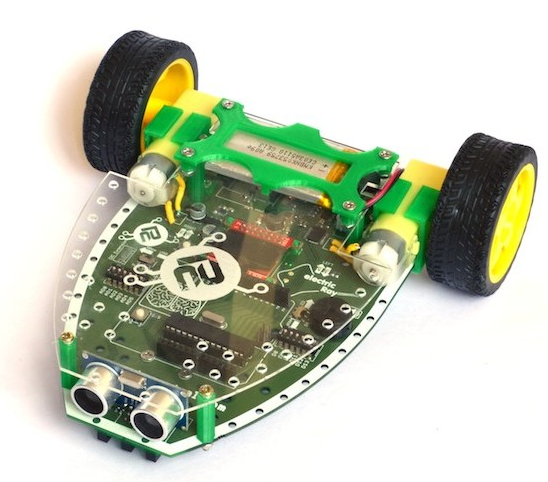
\includegraphics[scale=0.2]{Fig_05.png}
\caption{Electric Ray Robot}
\end{figure}

Students are introduced to object-oriented program paradigm, by modeling Electric Ray robot as an 'object' which has 'state'(what it has) and 'behaviors' (what it does). This mental visualization of real world things as objects helps them later to ease into an object oriented programming language like Java.

\begin{figure}[h]
\centering
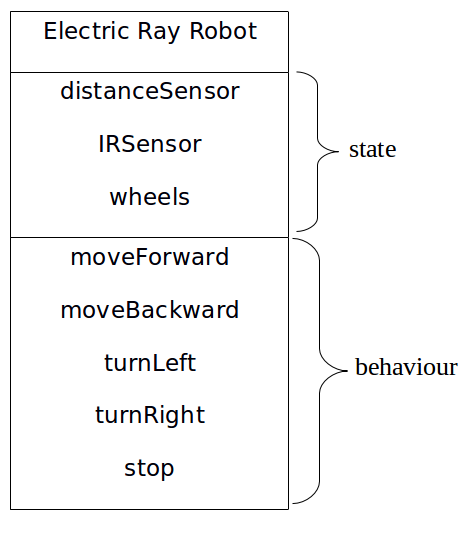
\includegraphics[scale=0.2]{Fig_06.png}
\caption{Object notation of Electric Ray}
\end{figure}

Behavioral State machines are diagrams which identifies the relation between above states and behaviors. Behavior changes the value of state of the object. For example, as the robot moves forward (behavior), distance sensor value (state) changes if an obstacle is in vicinity. Students model the behavioral state machine digaram for the problem in hand to get a diagramatic representation of the logic.

\begin{figure}[h]
\centering
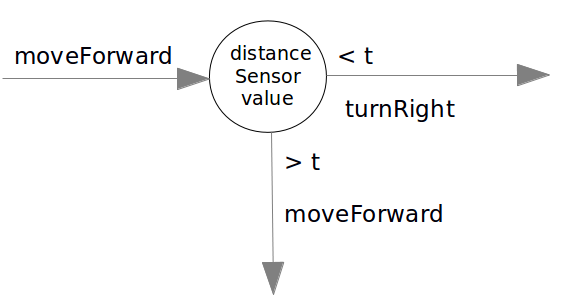
\includegraphics[scale=0.2]{Fig_07.png}
\caption{A behavioral state machine diagram}
\end{figure}

\thispagestyle{fancy}
\fancyfoot[R]{$^1$\textit{https://sites.google.com/site/electricrayprogramming/}}

\subsection{Programming fundamentals with Minibloq}
Minibloq is an open source graphical programming environment for Arduino, Multiplo, physical computing devices and robots. It consists of drag-and-drop blocks for the constructs used in programming. To solve a given problem, the blocks have to be arranged in a logical manner and then transferred to the robot via data cable. An advantage of Minibloq compared to other visual programming softwares is that it can be enhanced to add new blocks with functionality specific to your hardware. It can even be enhanced to support a new robot based on Arduino. The author had enhanced the software by abstracting the pin level details with new blocks specific for controlling the movement, sensors, display and buzzer of Electric Ray Robot.

\begin{figure}[h]
\centering
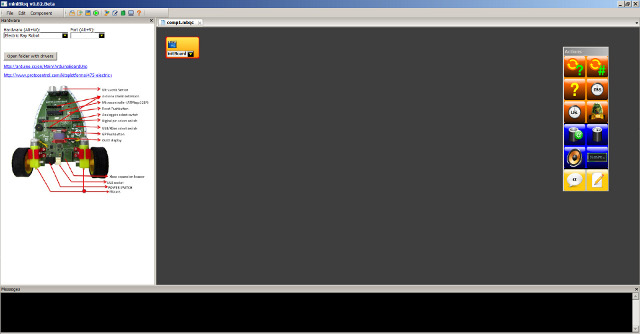
\includegraphics[scale=0.3]{Fig_08.png}
\caption{Minbloq programming environment}
\end{figure}

A manual$^1$ containing 10 sections which explains the concepts of variables, delays, if else statements, while loops, repeat loops, controlling the motors, sensors, buzzer and OLED display is hosted for the students. The manual also contains sample programs for each of the section. Last two sections are for advanced programmers and explains how to enhance Minibloq.

\begin{figure}[h]
\centering
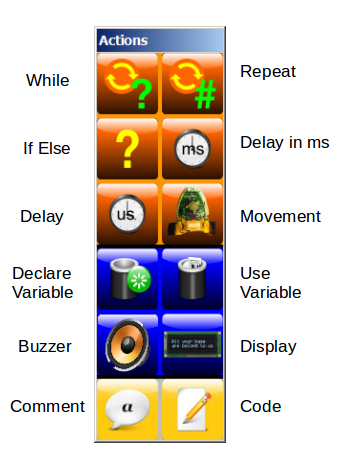
\includegraphics[scale=0.3]{Fig_09.png}
\caption{Minbloq drag-and-drop blocks}
\end{figure}

Once the different blocks are understood, it is very intuitive for students to write programs. To write a "Hello World" program, all that need to done is to drag and drop a block for OLED display, followed by a block to specify the data type (string text or numeric text), followed by the text.

\begin{figure}[h]
\centering
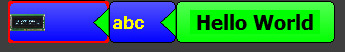
\includegraphics[scale=0.5]{Fig_10.png}
\caption{Hello World program in Minibloq}
\end{figure}

The program is ported to the robot and the output is displayed on its OLED.

\subsection{Advanced programming and development}
Minbloq converts the visual program to its corresponding arduino code. Once students are comfortable with the fundamentals, they can open the “Generate code” window in Minibloq to learn the code that is being generated. Minibloq also allows to type in actual code where they can practice the constructs of programming.

\begin{figure}[h]
\centering
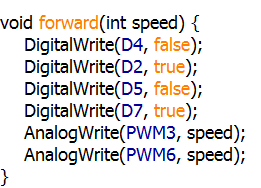
\includegraphics[scale=0.4]{Fig_12.png}
\caption{Code generated for forward block}
\end{figure}

What makes Minibloq unique from the other counter parts in visual programming is that it is open source and allows programmers to enhance it by adding new blocks. It also allows to configure a new robot with Minibloq. This can be easily done by programmers familiar with Arduino and embeded systems. Last two sections of the manual$^1$ explains this.

\section{Empirical Results}

\subsection{Square path Program}

The task involved is to make the robot move in square paths. Each time it takes a turn, it should increment a counter and display the value. This program helped to learn the concepts of variables and delays and how to use them in solving a problem. The amount of delay that is required for an accurate right turn is left for the students to experiment and find out.

\begin{figure}[h]
\centering
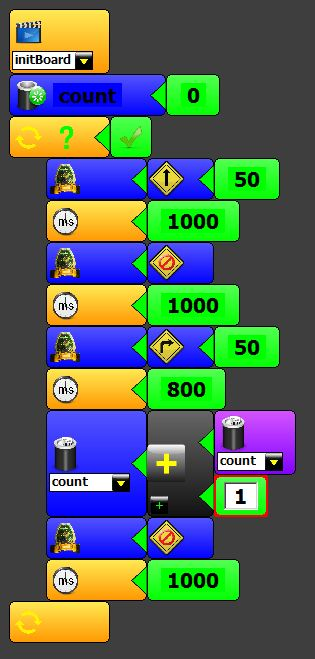
\includegraphics[scale=0.5]{Fig_13.png}
\caption{Square path Program}
\end{figure}

\begin{figure}[h]
\centering
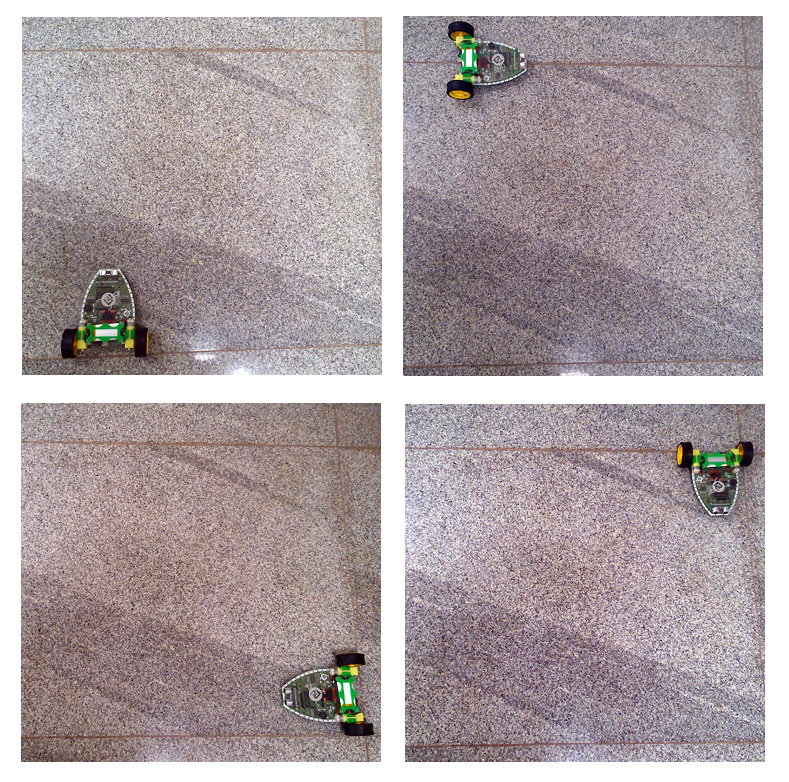
\includegraphics[scale=0.3]{Fig_15.png}
\caption{Square path Program Output}
\end{figure}

\subsection{Obstacle Sensor Program}

The task involved is to teach the robot sense an obstacle. While moving forward, if it senses an obstacle, the robot should sound the buzzer, stop and take a right turn. This program is as a good introduction to robotics where students can learn about sensors. Designing a maze and teaching the robot to find the way out the maze is another creative exercise using sensors.

\begin{figure}[h]
\centering
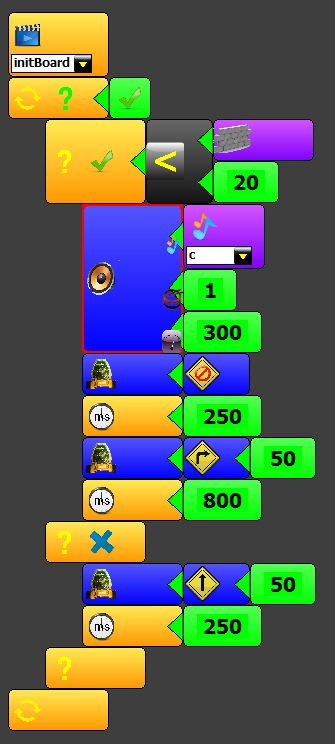
\includegraphics[scale=0.5]{Fig_14.png}
\caption{Obstacle Sensor Program}
\end{figure}

\begin{figure}[h]
\centering
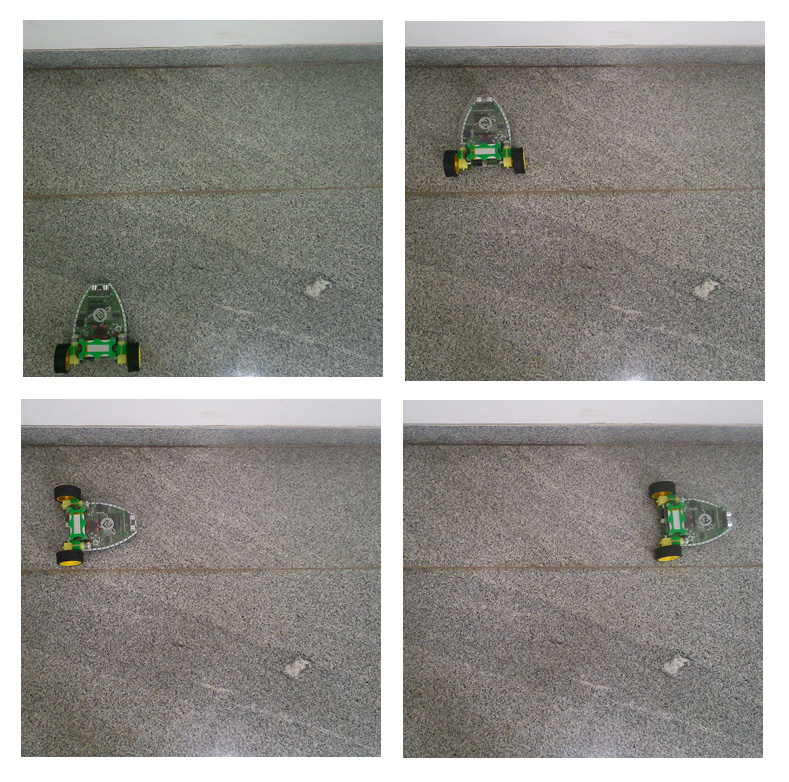
\includegraphics[scale=0.3]{Fig_16.png}
\caption{Obstacle Sensor Program Output}
\end{figure}

\subsection{Obstacle Sensor Block Development}

This task for advanced programmers involved understanding the obstacle sensor used in the robot and develop a block for it in Minibloq. The last two sections of the manual$^1$ explains how to develop a block for forward movement. Similar approach was used to develop a block for obstacle sensor.

\section{Conclusion and Future Work}

The author's institute conducts a program every year to motivate high school children on Information Technology. This model was demonstrated and received a favourable response from the students as well as the teachers. Once the students got introduced to Minibloq they could focus on logic for completing the given task rather than complaining about syntax and compilation errors. The involvement of a robot made it a fun filled task. 

In the future, a factor we like to improve on is the turn around time for completing each program. The porting of the program to the robot and testing it several times to get the correct version consumed time. This can be improved by building a virtual Electric Ray robot simulator to Minibloq where the students can test their trial programs. This would also involve building a physics engine simulated environment which can interact with the sensors of the virtual robot. So the students first test their program with the simulated robot and makes necessary corrections. Once the program with the simulator is successful, it can be ported to the physical robot to see the actual output.


\begin{thebibliography}{1}

\bibitem{karel} Richard E. Pattis, \emph{Karel the Robot A Gentle Introduction to the Art of Programming}, John Wiley \& Sons Inc., 1981

\bibitem{eray} http://www.protocentral.com/robotics-kits/475-electric-ray-robot.html

\bibitem{lego} Barry S. Fagin, Laurence D. Merkle, Thomas W. Eggers, \emph{Teaching Computer Science With Robotics Using Ada/Mindstorms 2.0}, ACM SIGAda Ada Letters, 2001

\bibitem{alice} Briana Lowe Wellman, James Davis, Monica Anderson, \emph{Alice and Robotics in Introductory CS Courses}, ACM New York, 2009

\bibitem{aerobot} Michael Rubenstein, Bo Cimino, Radhika Nagpal, \emph{AERobot: an Affordable Education Robots}, https://sites.google.com/site/affordableeducationrobot

\end{thebibliography}



\end{document}